\documentclass[letterpaper,11pt,oneside]{article}
%\documentclass[a4paper,11pt,oneside]{article}
 
\usepackage{multicol}

\usepackage{times}
\usepackage{epsfig}
 
\usepackage{verbatim}
 
%\usepackage[none,bottom,dark,english]{draftcopy}
%\draftcopyName{ DRAFT \number\day\/\number\month\/\number\year}
 
\usepackage[verbose]{geometry}
%\geometry{top=2cm,bottom=2cm,left=1.5cm,right=1.5cm,nohead}
\geometry{top=1in,bottom=1in,left=1in,right=1in,nohead}

\def\plotwidth{0.7\columnwidth}

%\setlength{\parindent}{0pt}
%\setlength{\parskip}{1.0ex plus0.5ex minus0.5ex}


\begin{document}

\title{Modelling and Shuffling: The significance of alignments and matches for
medium or low information sequences}
% ?models don't shuffle?  ha, ha

%\author{
%  David R. Powell
%}
\author{
  David R. Powell\footnotemark[1]~, Lloyd Allison and Trevor I. Dix \\
{\small powell@csse.monash.edu.au, lloyd@bruce.cs.monash.edu.au, trevor@csse.monash.edu.au} \\
  Member of the Victorian Bioinformatics Consortium and \\
  School of Computer Science and Software Engineering, \\
  Monash University, Australia 3800.}

\renewcommand{\thefootnote}{\fnsymbol{footnote}}
\footnotetext[1]{Partially funded by Australian Research Council Grant A49800558}
\renewcommand{\thefootnote}{\arabic{footnote}}

\date{}
\maketitle

%-------------------------------------------------------------------------

%\toappear{Submitted to the RECOMB-2003 refereeing process 30 September 2002.}

\begin{abstract}
An alignment methodology that incorporates general
population models into the alignment process is described.
It gives a better significance test than comparison with alignment of shuffled
sequences.
It places very few restrictions or requirements on the kind of
population model that can be used.
Tests show that accuracy at predicting relatedness is equivalent to
the standard shuffling technique on uniform random data and
is better on populations from higher-order and mixed (hidden) models;
there are fewer false-positives and false-negatives.
The rank-order of alignments of two given sequences can,
and should, be open to change compared to other methods.
The rank-order of matches between a query sequence and a collection of
sequences can, and should, also be open to change compared to other methods. 
\end{abstract}

{\small Keywords: sequence analysis, sequence alignment, information theory, compression}

%-------------------------------------------------------------------------
\section{Introduction}
\label{sec:intro}

Most alignment algorithms assume that sequences to be aligned are random,
or perhaps that they are well described by a zero-order Markov model.
It is well known that compressible sequences,
i.e. non-random sequences of medium or low information content,
often cause false positive matches with such algorithms.
Steps to address this problem include
comparing alignment results with those for shuffled sequences, and
masking-out sub-intervals of low information content.
Shuffling assumes a necessarily simple population model in the sense that it preserves low-order statistics.
Masking-out is drastic because it implies that
medium or low information equals zero information which is false.
We describe a different approach, {\em modelling-alignment} (M-alignment), which explicitly models
the statistical properties of populations of sequences and
gives the appropriate weight to each character in a sequence.
It can be used with a wide class of models of populations,
with few restrictions.
It allows models of differing complexities to be compared fairly and
it gives a natural significance test.
The rank-order of alignments, even for just two sequences, and
the rank-order (of alignments) of matching sequences for a query sequence
can in general
be changed by M-alignment, so both false-positives and also false-negatives can be reduced.
It is compared to the Smith-Waterman~\cite{smith81} program \verb!prss! (from the FASTA
package) which is based on \verb!rdf2!~\cite{pearson88}
with a significance test based on shuffling.
Results show that the two methods perform equally well on uniform, random data and
that M-alignment is in general more accurate on non-random (compressible) sequences.

There are many definitions for
distance, or conversely similarity, between two
sequences of values, e.g. DNA or protein sequences.
Given two sequences of lengths m and n,
the well known dynamic programming algorithm (DPA) (Figure~\ref{fig:algs}(a)) finds
optimal alignments for various cost or score criteria in O(m*n)-time,
for example the longest common subsequence (Figure~\ref{fig:algs}(b)) or
other scores (Figure~\ref{fig:algs}(c)).
Levenshtein~\cite{levenshtein66} gave a definition of what is now known as the
(simple) edit- or evolutionary-distance where point mutations
(change, insert or delete a character) each have a cost of one.
This metric was later studied by Sellers~\cite{sellers74} and many others.
The method and its algorithm (Figure~\ref{fig:algs}(d)) can be described as cost based, simple costs (0$|$1), global alignment.
Linear gap costs~\cite{gotoh82}, also known as affine gap costs, are more plausible in biology.
If mutation events occur with certain probabilities,
the DPA can be used to find a most-probable alignment (Figure~\ref{fig:algs}(e)).
The local alignment problem~\cite{sellers80} is to find
matching pairs of subintervals, one from each sequence.

Bishop and Thompson~\cite{bishop86} recognised that an alignment, optimal or not,
is just a hypothesis about how two sequences are related.
Two alignments are exclusive hypotheses so their probabilities
can be summed (Figure ~\ref{fig:algs}(f));
for numerical reasons it is better to work with -log probabilities (Figure~\ref{fig:algs}(g)).
Allison et al~\cite{allison92a} extended summed alignment to
3-state models (affine gap costs) and
5-state models (piece-wise linear gap costs),
and included the model complexity,
giving a hypothesis test based on information content.

Needleman and Wunsch~\cite{needleman70} described an algorithm to find good matches between
two (or more) protein sequences.
To assess the significance of the match score of two sequences
they compared it to scores obtained
when ``one member of the protein pair was randomized'', i.e. permuted, shuffled.
Permuting a sequence preserves the zero-order statistics,
i.e. the character frequencies, but
in general destroys higher-order statistics.
Powell et al~\cite{powell98b} and Allison et al~\cite{allison99} gave alternatives in which models
of populations of sequences are incorporated into the alignment algorithm
to weight characters appropriately.

The following sections first briefly review
simple v. affine gap-costs,
local v. global alignment, and
optimal v. summed alignment.
Modelling- (M-) alignment (Figure~\ref{fig:algs}(h)), where statistical properties of a
population are considered, is then defined in
local-alignment, global-alignment, affine-gapped, optimal-alignment and summed-alignment variants.
Finally it is compared to the standard Smith Waterman program plus shuffling
on various populations of sequences.
ROC curves (Figures~\ref{fig:roc_uni} to \ref{fig:roc_blend})
show M-alignment performs as well as the standard method on uniform 
random data, and better on more complex models.




\section{Gap Costs or Scores}

Simple point mutations rank $L$ separated point insertion (or deletion) events
the same as one event of $L$ contiguous insertions.
It is more plausible in biology to prefer the latter over the former and
this can be modelled by affine gap costs of the form $a \times L+b$ for
constants $a$ and $b$.
Constant `$a$' is a start-up penalty that applies pressure towards having
a low number of gaps.
Gotoh~\cite{gotoh82} gave an O(m*n)-time alignment algorithm for affine gap-costs.
The key idea is to introduce three {\em states} into  each cell of
the matrix used by the dynamic programming algorithm (Figure~\ref{fig:3state}).
The states represent the cost (probability, score, etc.) of reaching
element (i,j) {\em conditional} upon a
diagonal (match or mismatch), vertical (insert) or horizontal (delete) move.



\section{Local v. Global}

Sellers~\cite{sellers80} gave a precise definition for local alignment
of two sequences under the simple evolutionary (edit) distance:
``Two portions, one from each sequence, are similar if they are close
in the metric space of evolutionary distances. The method allows
a complete list to be made of all pairs of intervals,
one from each of two given sequences, such that each pair
displays a maximum local degree of similarity.''

A local alignment algorithm may be viewed as a global alignment algorithm on
{\em subsequences} where the start and end of the subsequences must also be determined.
This is illustrated in Figure~\ref{fig:local}.  In a global alignment
algorithm, each cell in the DPA matrix is calculated from its three
neighbouring cells (Figure~\ref{fig:algs}). In local alignment, this is
extended so that an alignment may start (or end) at any cell in the matrix.

The Smith-Waterman algorithm~\cite{smith81} is a standard,
much used alignment algorithm for comparison of biological sequences.
It is a local alignment
algorithm utilising affine gap costs.  This algorithm is defined in terms of
scores; positive for a match, and negative for a change and for gaps.  The
scores used in the Smith-Waterman algorithm are not unique, indeed, many
different sets of scores and also costs produce the same rank ordering of
alignments.  We make use of this by converting the Smith-Waterman scores to
probabilities for the initial mutation probabilities in our M-alignment
algorithm.


\section{Optimal v. Sum over all Alignments}

An alignment is just a hypothesis about how two sequences are related,
assuming that they are related.  If one alignment is ``true'' then
a different one must be ``false'' -- they are exclusive.
The probability of two related sequences is therefore the sum of
their probabilities over all alignments~\cite{bishop86}
if it accepted that the set of alignments represents all
possible ways of being related.
Allison et al~\cite{allison92a} extended this to 3-state (affine gap-costs)
and 5-state (piecewise-linear gap-costs) models and included
the model complexity which allowed simple and complex
mutation models to be compared fairly and gave a natural hypothesis test.
It is quite possible, for distantly related sequences, that any single
optimal alignment is not an acceptable hypothesis yet the total probability
over all alignments shows them to be related.
This is consistent with the observation of
Gribskov and Robinson~\cite{gribskov96} that there is
a ``fundamental difference between the searching [for related sequences]
and [optimal] alignment operations.''

Every alignment ``explains'' all the characters of the given sequences.
If a character constant, $c$, is added for every character
in every column of an alignment (or in every move in the DPA matrix)
this just adds a constant to the cost (or score) of the alignment.
It does not change the rank-order of alignments of two sequences.
The observation allows the normalisation of mutation costs into
probabilities~\cite{allison93a} (or the conversion of probabilities into other costs).
We shall argue later that changing the cost (score) of a character
{\em in a context} can, and sometimes should, change the rank-order
of alignments.


\section{Random v. Compressible}

We take the terms compressible, non-random, and low information content
to be equivalent as they apply to sequences, this being a consequence of
Shannon's mathematical theory of communication~\cite{shannon48}.
For example, if a DNA sequence is random, that is the probability of every
base in any context is 1/4, it is impossible to do better than to allocate
each base a fixed 2-bit code.
If something more is known about composition (zero-order statistics),
the tendency of one base to follow another (1st-order),
frequencies and run-lengths of poly-A or (AT)*, or
frequencies and similarities of ALU sequences~\cite{herzel94}, etc.,
then it is possible to predict the next base with greater than one success
in four and to design a code that is more efficient than 2-bits per base,
on average.  There is significant interest in compression of sequences for
pattern discovery~\cite{grumbach94, loewenstern97, rivals97, allison00a, stern01}.

It is well known that low-information content sequences tend to cause
false-positive matches in alignment algorithms that assume
the data to be random, or perhaps to come from a zero-order model.
Steps to cure the problem include
significance tests that compare results against shuffled sequences, and
the masking-out of repetitive subintervals~\cite{wootton93}.
Needleman and Wunsch~\cite{needleman70}
asked ``whether a particular [match score] found differs significantly
from a fortuitous match between two random sequences.''
And proposed that one ``construct two sets of random sequences,
from the amino acid composition of each of the proteins compared. ...
If the [match] value found for the real proteins is significantly different
from the values found for [two of] the random sequences,
the difference is a function of the sequences alone and
not of the compositions.''
We collectively call this technique and its later variations `shuffling'.

Randomly permuting a sequence preserves its zero-order statistics (composition)
but in general destroys higher-order statistics.
It is possible to shuffle a sequence while preserving its first-order
statistics and its codon usage~\cite{fitch83, altschul85} but
it is hard to see how to do this while preserving its statistics under
an arbitrary model.
Even when its assumptions hold,
shuffling is only a significance test which is only half of an answer:
One or more alignments are obtained and are then tested for significance;
the significance test can only rule an alignment out.
It may be that a truly significant alignment was given a low rank,
and was ignored by the alignment algorithm because it was
ignorant of any population model.
Shuffling cannot bring this false negative back into consideration.

In general, characters are not all equal and instances of a character
value may not be equal in different contexts.
For example, if `x' is rarer than most other letters in English text
then it is generally more important to match `x's than `e's, say,
in alignments of text because the former are {\em features}.
But if `x' is rather common after `e'
then `x' is much less important, unexceptional, in that context.
This kind of effect can be modelled by considering the probability
of a character {\em in context}, $Pr(a[i]=c|a[1..i-1])$,
i.e. by modelling populations of sequences.
By using (-log) probabilities of characters in context within the DPA
(e.g. Figure~\ref{fig:algs}(h)), characters are weighted appropriately and the DPA tries
to match important features and places less emphasis on common, chance matches.
In DNA a run of poly-A or (AT)*, or an ALU becomes less important than
mere length would suggest, of less but not of zero importance (information).
Modelling can and should change the rank-order of alignments,
even of just two sequences, and can reduce the chance of false-negatives.


\begin{figure}
\begin{minipage}{\textwidth}
\begin{multicols}{2}

\footnotesize
\begin{verbatim}
m[0,0] = z

m[i,0] = f(m[i-1,0],
           c(a[i],noCh)), i=1..|a|

m[0,j] = f(m[0,j-1],
           c(noCh,b[j])), j=1..|b|

m[i,j] = g(f(m[i-1,j-1],c(a[i],b[j])),
           f(m[i-1,j  ],c(a[i],noCh)),
           f(m[i,  j-1],c(noCh,b[j]))),
             i=1..|a|, j=1..|b|
\end{verbatim}

(a) Generic dynamic programming algorithm (DPA).


\begin{verbatim}
g = max
z = 0
f = +
c(x,x) = 1
c(x,y) = 0, x<>y
c(x,noCh) = c(noCh,y) = 0
\end{verbatim}

(b) Longest common subsequence (LCS).


\begin{verbatim}
g = max
z = 0
f = +
c(x,x), c(x,y), c(x,noCh) &
c(noCh,y) scores of choice
\end{verbatim}

(c) Arbitrary scores.


\begin{verbatim}
g = min
z = 0
f = +
c(x,x) = 0
c(x,y) = 1, x<>y
c(x,noCh) = c(noCh,y) = 1
\end{verbatim}

(d) Edit distance (0$|$1).


\begin{verbatim}
g = max
z = 1
f = *
c(x,x) = Pr(match)*Pr(x)
c(x,y) = Pr(mismatch)*Pr(x,y | x<>y)
c(x,noCh) = Pr(delete)*Pr(x)
c(noCh,y) = Pr(insert)*Pr(y)
\end{verbatim}

(e) Most probable alignment.


\begin{verbatim}
g = +
z = 1
f = *
c(x,x) = Pr(match)*Pr(x)
c(x,y) = Pr(mismatch)*Pr(x,y | x<>y)
c(x,noCh) = Pr(delete)*Pr(x)
c(noCh,y) = Pr(insert)*Pr(y)
\end{verbatim}

(f) Sum over all alignments.


\begin{verbatim}
g = logPlus where
  logPlus(-log(p1),-log(p2)) = -log(p1+p2)
z = 0
f = +
c(x,x) = -log(Pr(match))-log(Pr(x))
c(x,y) = -log(Pr(mismatch))-log(Pr(x,y|x<>y))
c(x,noCh) = -log(Pr(delete))-log(Pr(x))
c(noCh,y) = -log(Pr(insert))-log(Pr(y))
\end{verbatim}

(g) -log sum over all alignments.


\begin{verbatim}
g = max
z = 1
f = *
At m[i,j]:
 c(x,x) = Pr(match)*Pr(x|a[1..i-1],b[1..j-1])
 c(x,y) = Pr(mismatch)*
             Pr(x,y|x<>y,a[1..i-1],b[1..j-1])
 c(x,noCh) = Pr(delete)*Pr(x|a[1..i-1])
 c(noCh,y) = Pr(insert)*Pr(y|b[1..j-1])
\end{verbatim}

(h) Most probable alignment, non-random sequences.

\end{multicols}
\end{minipage}
\caption{\label{fig:algs}Summary of various 1-state, global alignment algorithms.}
\end{figure}

\begin{figure}
%\begin{minipage}{\textwidth}
\begin{multicols}{2}

%\begin{figure}
\centering
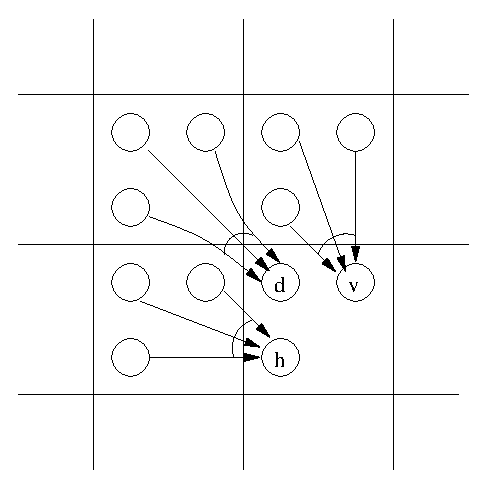
\epsfig{file=3state.eps, width=0.8\columnwidth}
\caption{\label{fig:3state}DPA for affine gap costs aka. 3-State mutation model.}
%\end{figure}

\pagebreak

%\begin{figure}
\centering
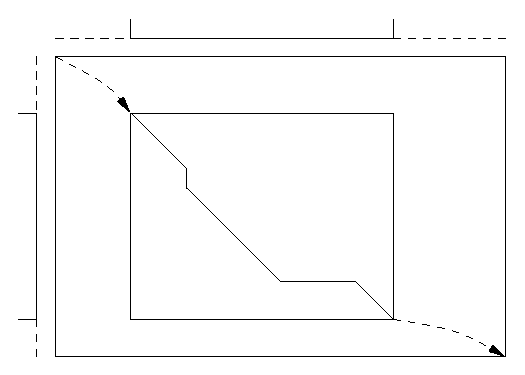
\epsfig{file=local.eps, width=0.7\columnwidth}
\caption{\label{fig:local}Local alignments}
%\end{figure}

\end{multicols}
%\end{minipage}
\end{figure}


\section{Description}

The aim of probabilistic optimal alignment is to find the probability of the
sequences and the most probable alignment.  Summing over all alignments aims
to calculate the probability of both sequences given they are related by an
alignment model.  For practicality -log probabilities are used which directly
relates to a possible encoding length~\cite{shannon48}.  Much of the following
discussion alternates between probabilities and encoding length, using
whichever is more appropriate at the time.

When testing for the relatedness of sequences, we are really testing for
whether each sequence contains information about the other sequence.  For two
sequences, $A$ and $B$, by encoding both sequence under all possible alignment
we are attempting to determine their joint probability, $P(A \& B)$.  We can
also encode the sequences independently to calculate $P(A) \times P(B)$, also
known as the null model.  The ratio in these probabilities, $P(A \& B) / (P(A)
\times P(B))$, alternatively, by taking logs, the difference in the encoding
length from the null model and the alignment model, quantifies which model is
a better description of the data and by how much.  If we are able to use the
correct population model in calculating $P(A\&B)$, then difference in encoding
length indicates exactly how much information the sequences contain about each
other.  We refer to this difference as the log-odds ratio and it is the metric
for our tests. Using the wrong population model, or implicitly assuming a
uniform model, may cause us to overestimate the joint probability leading to
false positives.
\newpage
The new M-alignment algorithm is as shown in Figure~\ref{fig:algs}(h), using
the following probabilities for characters:
\begin{eqnarray*}
Pr(x|a[1..i-1],b[1..j-1]) & = & \frac{1}{2} ( Pr(a[i]|a[1..i-1]) +
Pr(b[j]|b[1..j-1]) ) \\
Pr(x,y|x<>y,a[1..i-1],b[1..j-1]) & = & \frac{1}{2}\frac{Pr(a[i]|a[1..i-1])
Pr(b[j]|b[1..j-1])}{(1-Pr(a[i]|b[1..j-1]))(1-Pr(b[j]|a[1..i-1]))}
\end{eqnarray*}

This version of the algorithm is for global alignment with a point mutation
model.  This is readily extended to affine gap costs by including three states
in each cell of the DPA matrix as shown in Figure~\ref{fig:3state}.  The
extension to local alignment is achieved by allowing an alignment to start at
any cell, $m[i,j]$, in the matrix with a probability of $P(a[1..i-1]) \times
P(b[1..j-1])$.  And an alignment may end at any point carrying a probability
of $P(a[i+1..|a|] | a[1..i]) \times P(b[j+1..|b|] | b[1..j])$.  For comparison
to existing techniques we will focus on local alignment using affine gap
costs.  When measuring the relatedness of two sequences, we sum over all
alignments as this is a better test than simply using the optimal alignment.

It is necessary for the encoding of the alignment to include any changeable
parameters so it is fair comparison between the null model and the alignment
model.  For affine gap costs M-alignment encodes the probabilities for each of
the different types of mutations.  Hence, it is possible to compare different
mutation models.  This may be useful in testing whether a point mutation
model, an affine gap model or a piece-wise linear model is best for some given
sequences.

The M-alignment algorithm starts with probabilities for mutations based on
those commonly used for the Smith-Waterman algorithm.  After one pass by the
algorithm, these parameters are re-estimated and the process repeated until
the encoding of the alignment converges to some minimum.  It is interesting to
note that the final estimated mutation probabilities are different depending
on whether optimal alignment or summed alignment is being done.
% -- Of course optimal-alignment gives biased parameter estimates,
% -- see Reconstruction of Strings Past,  maybe discuss in a jrnl version?


\subsection{Population models}

The type of population model required by the M-alignment algorithm is one that
can give a probability $P(a[i]=c|a[1..i-1])$ for every position $i$ in a
sequence.  This is sometimes known as a left-to-right sequence model and is
quite general.  The types of models tested in this paper are small order
Markov Models and mixtures of these, but there is no reason more complex models
could not used.  Indeed, the best model to use would be one that accounts for
all known structure in a population of sequences.

It is possible to use adaptive models.  However, such a model takes some time
to adapt to the sequence, so characters at the start of the sequence are
generally encoded with more bits than characters towards the end.  Hence, the
alignment algorithm may attempt to align characters at the start of the
sequences more carefully than characters at the end.  For this reason it is
best to use a fitted model instead of an adaptive model.

\subsection{Encoding of lengths}

When performing local alignment, for the encoding of the alignment to be a
correct encoding, it is necessary to encode at which position in both
sequences the alignment begins and ends.  We assume that the lengths of the
two sequences being compared are encoded independently, which seems sensible
for local alignments.  Since, we are interested only in the difference between
the null model and the alignment model and both would encode lengths in the
same way, we may ignore them.

However, it is necessary to encode the beginning and end of the alignment in
both sequences.  Since we assume the sequence lengths have already been
encoded, and we have no other prior knowledge on where the aligned section
will be in each sequence we use a uniform prior on the start and end position
of the aligned section.  Actually, we can do a little better than this.  Once
the start and end of one aligned subsequence is known and the start of other
subsequence is known, we have some knowledge about where the end of the second
subsequence will be.  This is due to the fact that the two aligned
subsequences will tend to be of similar length.  So, as an approximation, we
don't encode this final position at all.  This is a slight underestimate, but
is reasonable.  To be precise, if $l1$ is the length of the shorter sequence
and $l2$ the length of the longer, we encode the lengths of the un-aligned and
aligned regions in $2\log_2(l1) - 1 + \log_2(l2)$ bits.



\section{Tests}

Artificial data was used to compare the new M-alignment algorithm with the
common Smith-Waterman algorithm using shuffling as a significance test.  The
benefit of using artificial data is that the conditions can be controlled
precisely to clearly illustrate the advantages and disadvantages of
techniques.
We also know what the answer is.

The implementation used for the Smith-Waterman algorithm was the \verb!prss!
program that is part of the FASTA 3.3 package.  In all tests, the \verb!prss!
program was used with the standard parameters: +5 for a match, -4 for a
mismatch, -16 and -4 for the first and subsequent characters in a sequence
respectively.  The default of 200 uniform shuffles was used to determine the
significance of each alignment.

The artificial data was generated using a number of different population
models.  In all cases, 10 parent sequences were generated from the population
model(s).  Each parent sequence was generated to be of the form $gen(50\pm50)
.. gen(120\pm30) .. gen(100\pm50)$.  Where $gen(x\pm y)$ means to generate a
sequence with length selected uniform randomly from the range $[x-y, x+y]$.
Then from each parent, 25 child sequences were generated having only the
(mutated) middle sequence in common.  Of these 25 children, 5 were generated
by making 30 mutations, 5 by making 40 mutations, 5 with 50 mutations, 5 with
60 mutations and 5 with 80 mutations.  The exact method used for these
mutations is interesting in itself, but distracting at this point, the details
are given in Appendix~\ref{sec:mutations}.  The child sequences were
considered as the library to be searched, and each parent was used in turn as
the query sequence.  Thus for each query there were 25 related sequences of
differing relatedness and 225 unrelated sequences.  This ratio of related to
unrelated sequence in the library is a high compared to real sequence
databases but will suffice for testing purposes.  Each parent sequence was
compared against every child sequence making 2500 pair-wise comparisons.  Of
these 2500 comparisons, 250 are between related sequences, and 2250 between
unrelated sequences.

To present the results of the tests Receiver Operating Characteristics (ROC)
(\cite{gribskov96, brenner98}) plots are used.  Each algorithm tested produces
a number measuring the relatedness of the two sequences being compared.  This
may be the raw Smith-Waterman score, or the p-value found by the \verb!prss! 
program, or the log odds ratio produce by M-alignment.  For each test, the
2500 pair-wise comparisons are ranked in order of significance by this
measure.  For each possible cut-off value the number of true positives and the
number of false positives are counted.  Plotted on the y-axis is the ratio of
false positives to the total number of unrelated pair-wise comparisons.  And
on the x-axis the ratio of true positives to the total number of related
comparisons.  The better an algorithm is at separating related from unrelated
sequences the closer its curve will be to the bottom right corner of the ROC
plots.  Since we are mostly interested in the behaviour for a smallish number
of false positives the y-axis is plotted with a log scale.

In the first test, the population model is the simplest possible, a uniform
model.  That is, each character occurs with a probability of 1/4.  The ROC
plot in Figure~\ref{fig:roc_uni} shows that the \verb!prss! program, the raw
Smith-Waterman score and the M-alignment algorithm perform similarly.  This
test is relatively uninteresting and is only presented to show that for high
entropy sequences M-alignment performs like existing algorithms.  Recall that
M-alignment may take as a parameter the model for the sequences.  Except where
noted otherwise, the M-alignment algorithm is told to fit a 1st order Markov
Model to the sequences.


The next test is for sequences with a biased composition, that is, sequences
from a 0th order Markov Model.  The model chosen has an entropy of 1.76 bits
per character.  The shuffling method of the \verb!prss! algorithm is designed
to account for this type of alphabet bias, and indeed, as seen in
Figure~\ref{fig:roc_0} the performance of the \verb!prss! program and our
algorithm is similar.  Also, as expected, the raw score from the
Smith-Waterman algorithm does not do a very good job at separating the related
from unrelated sequences in this case.  Since the alphabet is essentially less
that 4 here, all algorithms have more difficulty in detecting relatedness than
in the previous test.


Figure~\ref{fig:roc_uni_0} shows the results for the next test.  In a sense,
this test is a combination of the previous two.  Instead of all 10 parent
sequences coming from the same population model, 5 come from a uniform model
(like the first test), and 5 from a 0th order Markov Model (like the second
test).  The shuffling of the \verb!prss! program does account for sequences
with a biased composition, but as seen in this test it does not perform as
well as M-alignment when there are different models in the population.
Similar behaviour has been seen when using other combinations of models.

%It may be argued that in practice the \verb!prss! program wouldn't use
%shuffling, but would use the results of all the database searches to fit the
%extreme value distribution.  NOT SURE WHAT AFFECT IT WOULD HAVE ON THIS
%TEST???   [Neither am I.]

The final test illustrates the benefits if one is able to better model the
population.  The population model in this test is a little more complicated.
This model consists of two sub-models.  One is a simple uniform model, and the
other a very biased 1st order Markov Model that produces sequences of
characters that are TATA-rich.  Sequences are generated by
choosing one of these two sub-models at random, then using that sub-model to
produce a random number of characters.  This is repeated a number of times to
% -- What is the "random number of characters" ???
produce a sequence of sufficient length.  This model is, in a sense, a blend
between a uniform model, with an entropy of 2 bits per character, and a 1st
order model, with an entropy of 1.1 bits per character.
Figure~\ref{fig:roc_blend} shows the results of the different algorithms on
sequences of this type.  Our algorithm is performing significantly better than
the \verb!prss! program.  The best performer in this figure is the M-alignment
algorithm using the ``blendModel''.  This blendModel was designed with some
knowledge of the population model.  Specifically, the blendModel knows that
the data is produced by a combination of a uniform model and also the exact
1st order model used.  It does not know the probability with which these
sub-models are chosen, nor the length of the sequences produced by the
sub-models.  As can be seen in the figure, having this extra knowledge about
the population model allows for better separation of related and unrelated
sequences.  The M-alignment algorithm is superior to the Smith-Waterman
algorithms because an arbitrary left-to-right sequence model can be used.
Thus, more complex population models may be used with M-alignment to allow
better differentiation between related and unrelated sequences.


It may be argued that this test is unfair to the \verb!prss! program since it
would be common practice to mask out low-complexity regions before doing the
comparison with the \verb!prss! program.  However, these low-complexity
regions do give \emph{some} information about whether the sequences are
related, just not as much information as high-complexity regions.

%INTERESTING THAT WE DO \emph{SO} WELL IN THIS ONE COMPARED TO PREVIOUS TESTS???
% Not particularly surprising? -- knowledge = power.


It is clear from the ROC plots that M-alignment is superior to
the \verb!prss! program when sequences are of low complexity, even when it is
simply a mixture of uniform and biased composition sequences.  However, the
\verb!prss! program performs well on these types of sequence if the population
is confined to one type.  This may be explained because the \verb!prss!
program does not have a natural cut-off p-value, and indeed the best cut-off
depends on the type of the population.  M-alignment has a natural cut-off at a
log-odds ratio of zero.  At zero, both the null model and the alignment model
are equally good explanations of the data.  In practice, a slightly larger
cut-off value would be used; a cut-off of 3 bits indicates the alignment model
is 8 times better than the null model, a cut-off of 10 bits gives a confidence
of about 99.9\% provided population model assumptions are appropriate.

The table below summarises the performance of the algorithms for a fixed
cut-off over the same data as the previous four tests.  The cut-off used for
M-alignment was 0, and for the \verb!prss! program $p=10^{-5}$ was used as
this seemed to do best over all.  In all cases the number of truly related
sequences is 250 (some very distantly related), and of unrelated 2250.
M-alignment performs in a similar manner as the \verb!prss! program in the
first test, and performs better in the others, considerably so in the second
and third.  The fourth test is interesting.  Recall from
Figure~\ref{fig:roc_blend} that the M-alignment algorithm achieves very good
separation of the related and unrelated sequences.  However, the true versus
false positives in the table below are not so good in all cases.  This is
because the model used with M-alignment is not the same as that used to
generate the data.  In the case where the blendModel is used, the entropy of a
sequence is over-estimated slightly.  But when a 1st order Markov model is
used in M-alignment, the entropy is over-estimated more.  So, while the method
still does a good job of separating the true positives from false positives, a
cut-off of 0 is not ideal in this case.  This is because some of the apparent
similarity between the sequences is really due to the population model, not to
sequences being related.  This highlights the fact that one should use the
best population model possible when aligning sequences. Knowledge, i.e. a good
model, is power and a poor model reduces power. Note that the best of two or
more alternative models can be detected on the basis of compression.

%\begin{minipage}{\textwidth}
\begin{center}
%\footnotesize
\begin{tabular}{|l|c||c|c|} \hline
Test set & Algorithm & true positives & false positives \\ \hline
Uni &  prss & 195 & 0  \\ 
Uni & Sum & 226 & 14  \\ \hline

0-order & prss & 89 & 0  \\ 
0-order & Sum & 211 & 17  \\ \hline

Uni \& 0-order & prss & 160 & 0  \\ 
Uni \& 0-order & Sum & 222 & 9  \\  \hline

Blend Uni \& 1-order & prss & 224 & 135  \\ 
Blend Uni \& 1-order & Sum (default 1st order) & 248 & 957 \\ 
Blend Uni \& 1-order & Sum (blendModel) & 246 & 116 \\ 
\hline \end{tabular}
\end{center}
%\end{minipage}




\section{Conclusion}
\label{sec:conc}


Modelling-alignment has been defined in local-, global-, affine gap-cost-,
optimal- and sum-of-all-alignment forms.  It incorporates a model of the
population of sequences into alignment algorithms and may be used with any
sequence model that can deliver $Pr(a[i]=c|a[1..i-1])$, mixture models and
hidden models included.  M-alignment gives weights to characters appropriately
depending on context; the rank-order of alignments can and should be open to
change, compared to other methods, as a consequence.  Its time-complexity is
the larger of O(m*n) and the time-complexity of the population model's
inference algorithm, i.e. usually O(m*n).  It is suggested that local- (or
global-), sum-of-all-, M-alignment be used to determine relatedness and that
optimal-, M-alignment be used to find an optimal alignment {\em given}
relatedness of the sequences.

M-alignment in global- and local-, sum-of-all-alignment form performs well
at predicting relatedness for various kinds of population.
Accuracy is equivalent to the standard Smith Waterman program with shuffling
on uniform random populations;
it is hard to see how a significance test based on shuffling could
cope well with arbitrary models of populations.
M-alignment performs better, as shown by ROC curves,
for compressible (non-random) populations if the true
population model, or a good model, is known.
It can perform badly if a bad model is used, as is to be expected,
but it can detect the better of two or more population models
on the basis of compression.

M-alignment can be used practically to determine relatedness
in small or moderate collections of sequences.
It could also be used on a client-computer to post-process, and re-rank,
putative matches returned from a large collection of sequences
by a fast search algorithm running on a server.
The latter use could reduce false-positives but not bring back
any false negatives.


%\begin{figure}
%\begin{minipage}{\textwidth}
%\begin{multicols}{2}

\clearpage

\begin{figure}
\centering
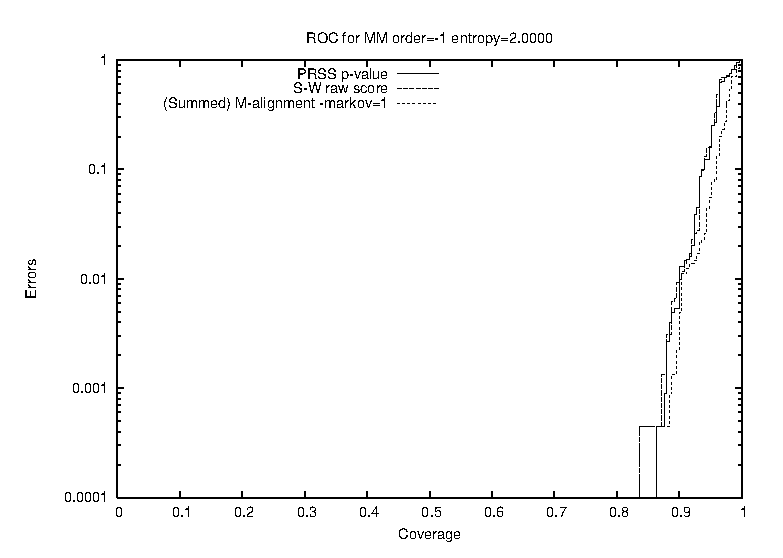
\epsfig{file=roc_uni.eps, width=\plotwidth}
\caption{\label{fig:roc_uni}ROC for a uniform sequence model.}
\end{figure}

\begin{figure}
\centering
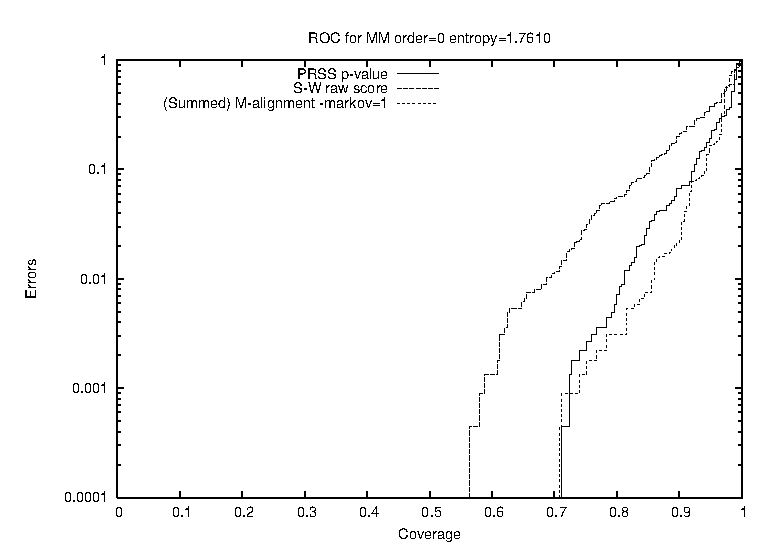
\epsfig{file=roc_0.eps, width=\plotwidth}
\caption{\label{fig:roc_0}ROC for biased composition sequences.}
\end{figure}

\begin{figure}
\centering
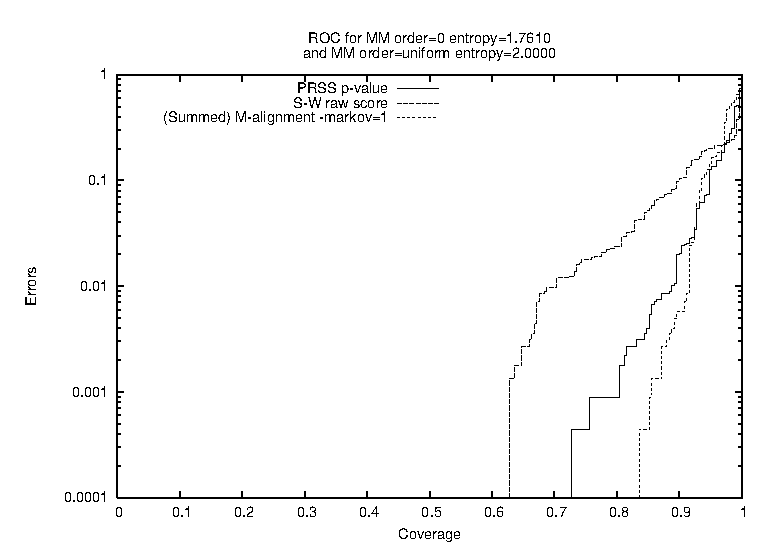
\epsfig{file=roc_uni_0.eps, width=\plotwidth}
\caption{\label{fig:roc_uni_0}ROC for a uniform sequence model and biased composition sequences.}
\end{figure}

\begin{figure}
\centering
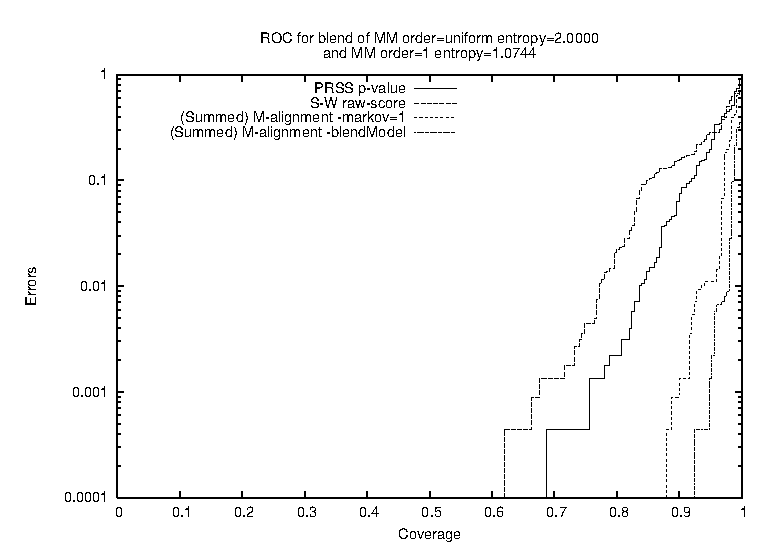
\epsfig{file=roc_blend.eps, width=\plotwidth}
\caption{\label{fig:roc_blend}ROC for a blended model}
\end{figure}

%\end{multicols}
%\end{minipage}
%\end{figure}

\clearpage

\bibliographystyle{abbrv}
%\bibliographystyle{alpha}
%\small
\bibliography{biblio}
%\normalsize


\appendix
\section{Mutation Model}
\label{sec:mutations}

When using a population model for sequences the problem arises of how to
mutate a sequence from this model such that the mutated sequence still
``fits'' the population model.  If characters are inserted, deleted or changed
without regard to the population model, the resulting mutated sequence will
tend towards a uniform population model.

We have a sequence, $A$, and a population model $M$.  The entropy of $A$ under
this model shall be written $M(A)$.  The length of sequence $A$ will be
written $|A|$.  The sequence that results from making $x$ mutations to $A$
shall be referred to as $A_x$.  We earlier described the motivation as wanting
the mutated sequence to ``fit'' the population model.  To make this precise,
what is desired is that as $x$ tends to infinity, the entropy of the mutated
sequence, $M(A_x)$, will tend to the entropy of the population model, $M$,
itself.

The method used to mutate sequences was inspired by the Metropolis
algorithm~\cite{metropolis53}.  Consider every possible sequence as having a
node, $S_i$ in a graph.  An arc between two nodes, $S_i$ and $S_j$, implies
that a single mutation relates the two corresponding sequences.  As we make
mutations to a sequence, we move between nodes in the graph.  In the extreme
case where many mutations are made, we want to visit each node with a
frequency equal to probability $p$, where $p$ is probability of that node's
sequence under the population model.  A sufficient condition for this is to
have the probability of taking the arc from $S_i$ to $S_j$ equal to the
probability of taking the arc from $S_j$ to $S_i$.

We will assume a point mutation model for simplicity.  That is, we consider
making mutations of the form delete a character, insert a character or change
a character.  For an alphabet of 4 characters, sequence $A$ has $3\times|A|$
possible change mutations, $|A|$ possible delete mutations and
$4\times(|A|+1)$ possible insert mutations.  If we assume a uniform, or
relatively flat, prior on the length of sequences, then we have the
requirement when mutating a sequence that on average the number of deletions
should be the same as the number of insertions.  There is a degree of freedom
in choosing the ratio of changes to insertions and deletions.  We shall use a
probability parameter $P_{change}$ for this.  We define two other probabilities
in terms of this.

\begin{eqnarray*}
P_{insert} & = & \frac{(1-P_{change})(4\times(|A|+1))}{(5\times|A|+4)} \\
P_{delete} & = & \frac{(1-P_{change})}{(5\times|A|+4)}
THERE IS AN ERROR HERE  should be (1-Pchange) / (5 + 4/len)
\end{eqnarray*}

When we mutate sequence $A$, a random choice is made whether to consider an
insertion, a deletion or a change mutation using the three above probabilities
(note they sum to unity).  If a deletion is to be considered, then the
position of the deletion is chosen uniform randomly over the length of the
sequence.  If a change, then the position and character are chosen randomly.
If an insertion, then the position and the character to be inserted are
randomly selected.  The sequence that would result from this mutation is $A'$.
Let $q$ be the probability given to sequence $A$ by the population model, and
$q'$ the probability given to sequence $A'$.  If $q'$ is greater than $q$ then
the mutation is accepted and $A'$ becomes $A_1$.  Otherwise, the mutation is
accepted with probability $q'/q$.  This process is repeated until the desired
number of mutations has been made.

The process of calculating $q'$ from the potential mutation can be done
efficiently if the population model $M$ is such that it operates on a local
level.  That is, if $q'$ can be calculated from $q$ and the potential mutation
in constant time.  This is true for fixed order Markov Models.

Since this method does not preclude a mutation ``undoing'' previous mutations,
the resulting mutated sequence, $A_x$, may be more similar to $A$ than
otherwise expected.  This tends to be more likely if $M$ is a very low entropy
model.

In the blendModel tests we make mutations as if the population model were a
uniform model.  Thus the more a sequence is mutated the higher its entropy
will become on average.  It is possible to use the method described above to
perform population mutations correctly.  Indeed, it could done efficiently
provided information were kept about which regions of the sequence came from
which sub-model.


%\section{STUFF TO BE DONE} 
%\begin{itemize}
%\item Reference these.
%\begin{itemize}
%\item linear gaps. \cite{altschul86}
%\item Extreme value stats for alignments \cite{karlin90}
%\item Blast+. \cite{altschul97}
%\end{itemize}
%\item Mention MML?
%\item Mention extreme value distribution, its use, and how we don't use it.
%\end{itemize}


\end{document}

